\section{Figure gallery}
\label{app:gallery}

Every figure in this appendix is drawn from committed run artifacts by
\texttt{scripts/report/} (no retraining) and is also in
\texttt{results/report/figures/}. Colours follow one fixed family palette, checked for
colour-vision deficiency; families are also distinguished by marker and position.
Circuits have one copy and runs use seeds 0--4 unless stated.

\begin{figure}[htbp]
  \centering
  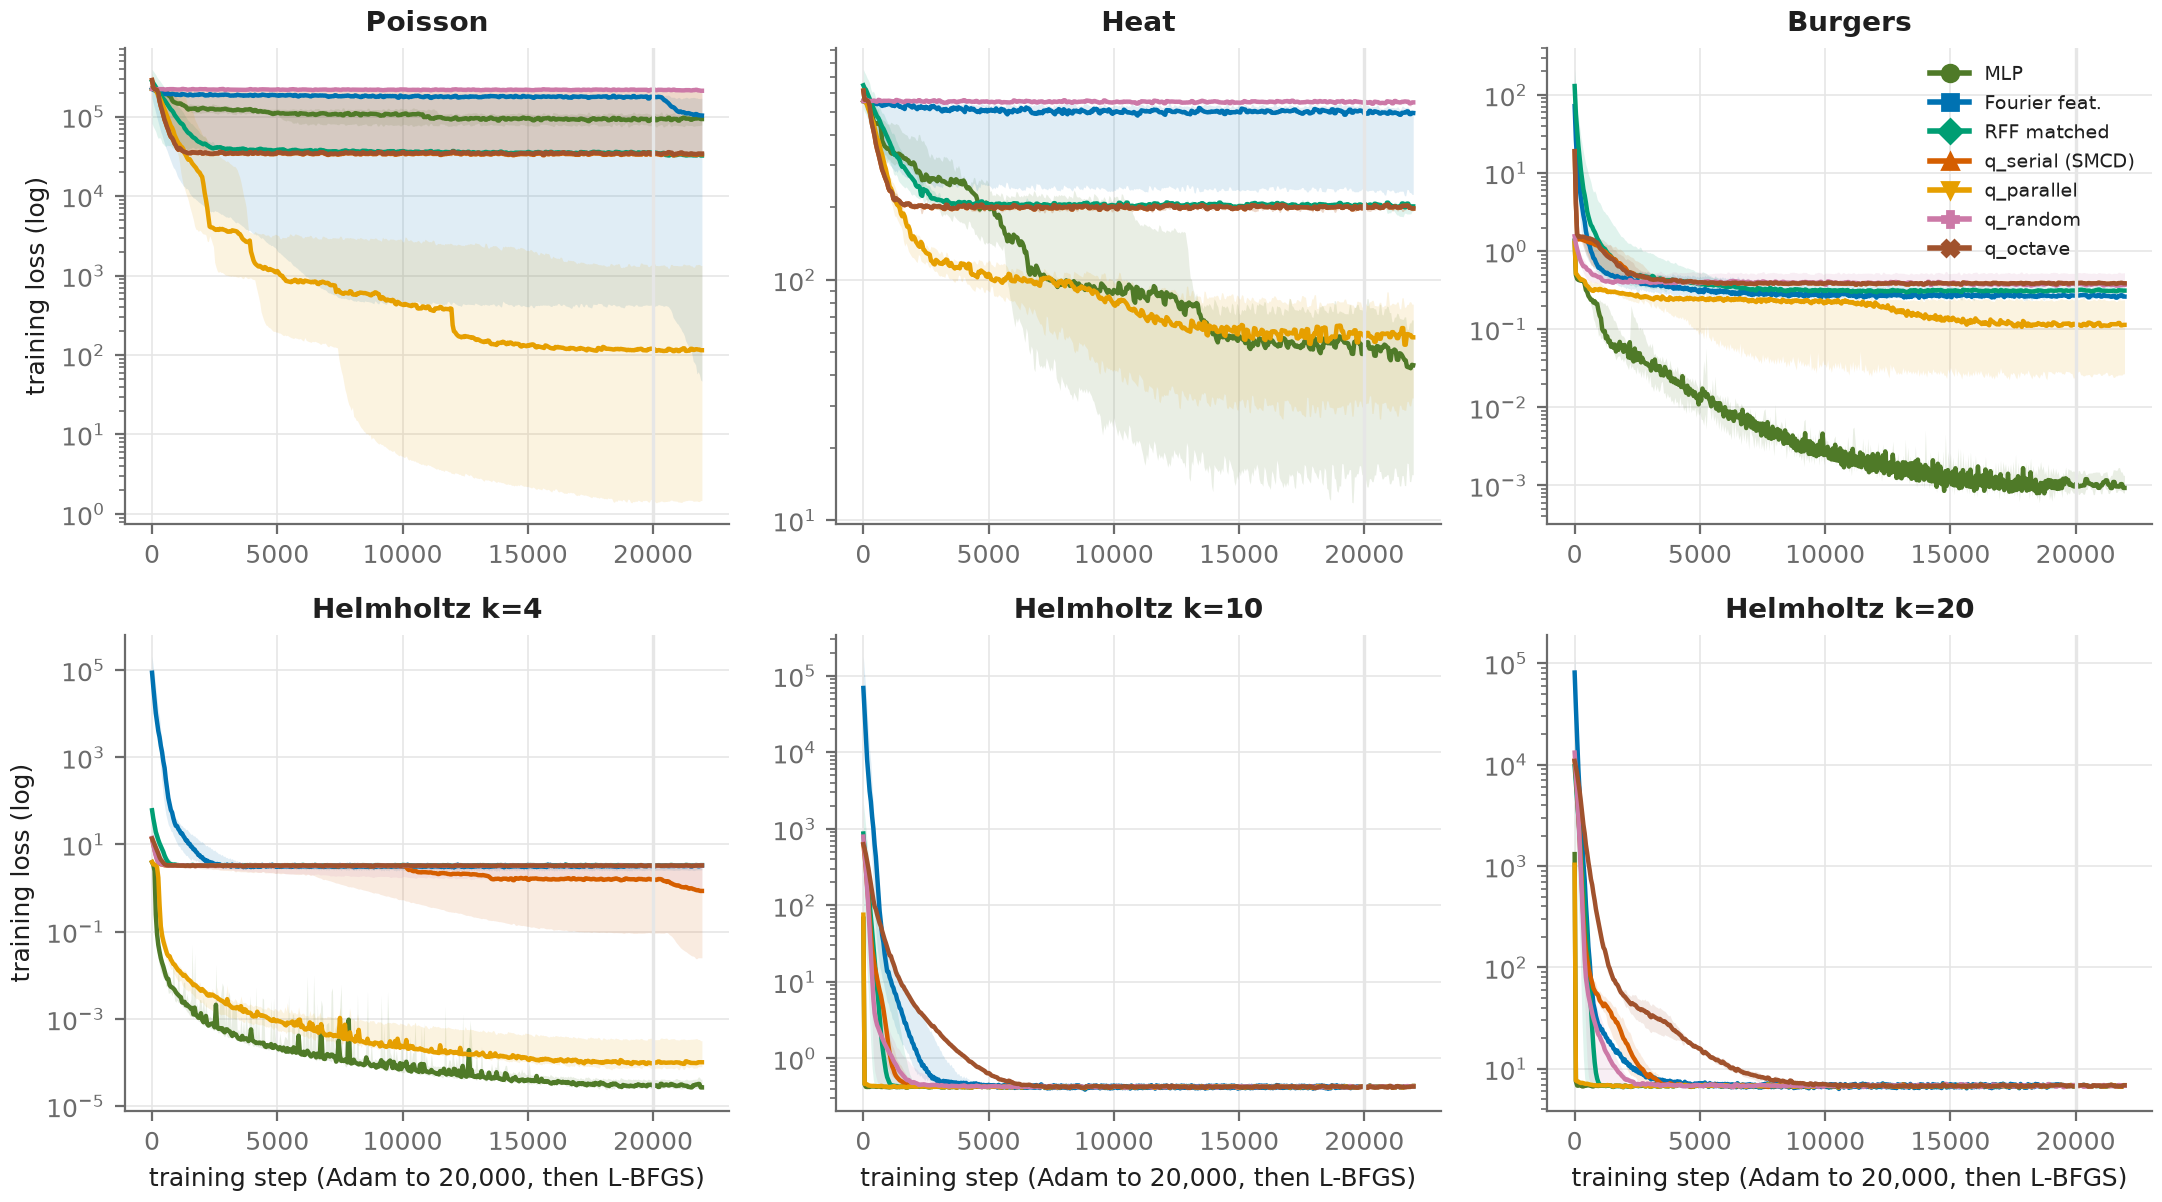
\includegraphics[width=\linewidth]{../results/report/figures/training_curves.png}
  \caption{Training loss, median over seeds with the seed range shaded. Adam runs to step
    20{,}000, then L-BFGS.}
  \label{fig:curves}
\end{figure}

\begin{figure}[htbp]
  \centering
  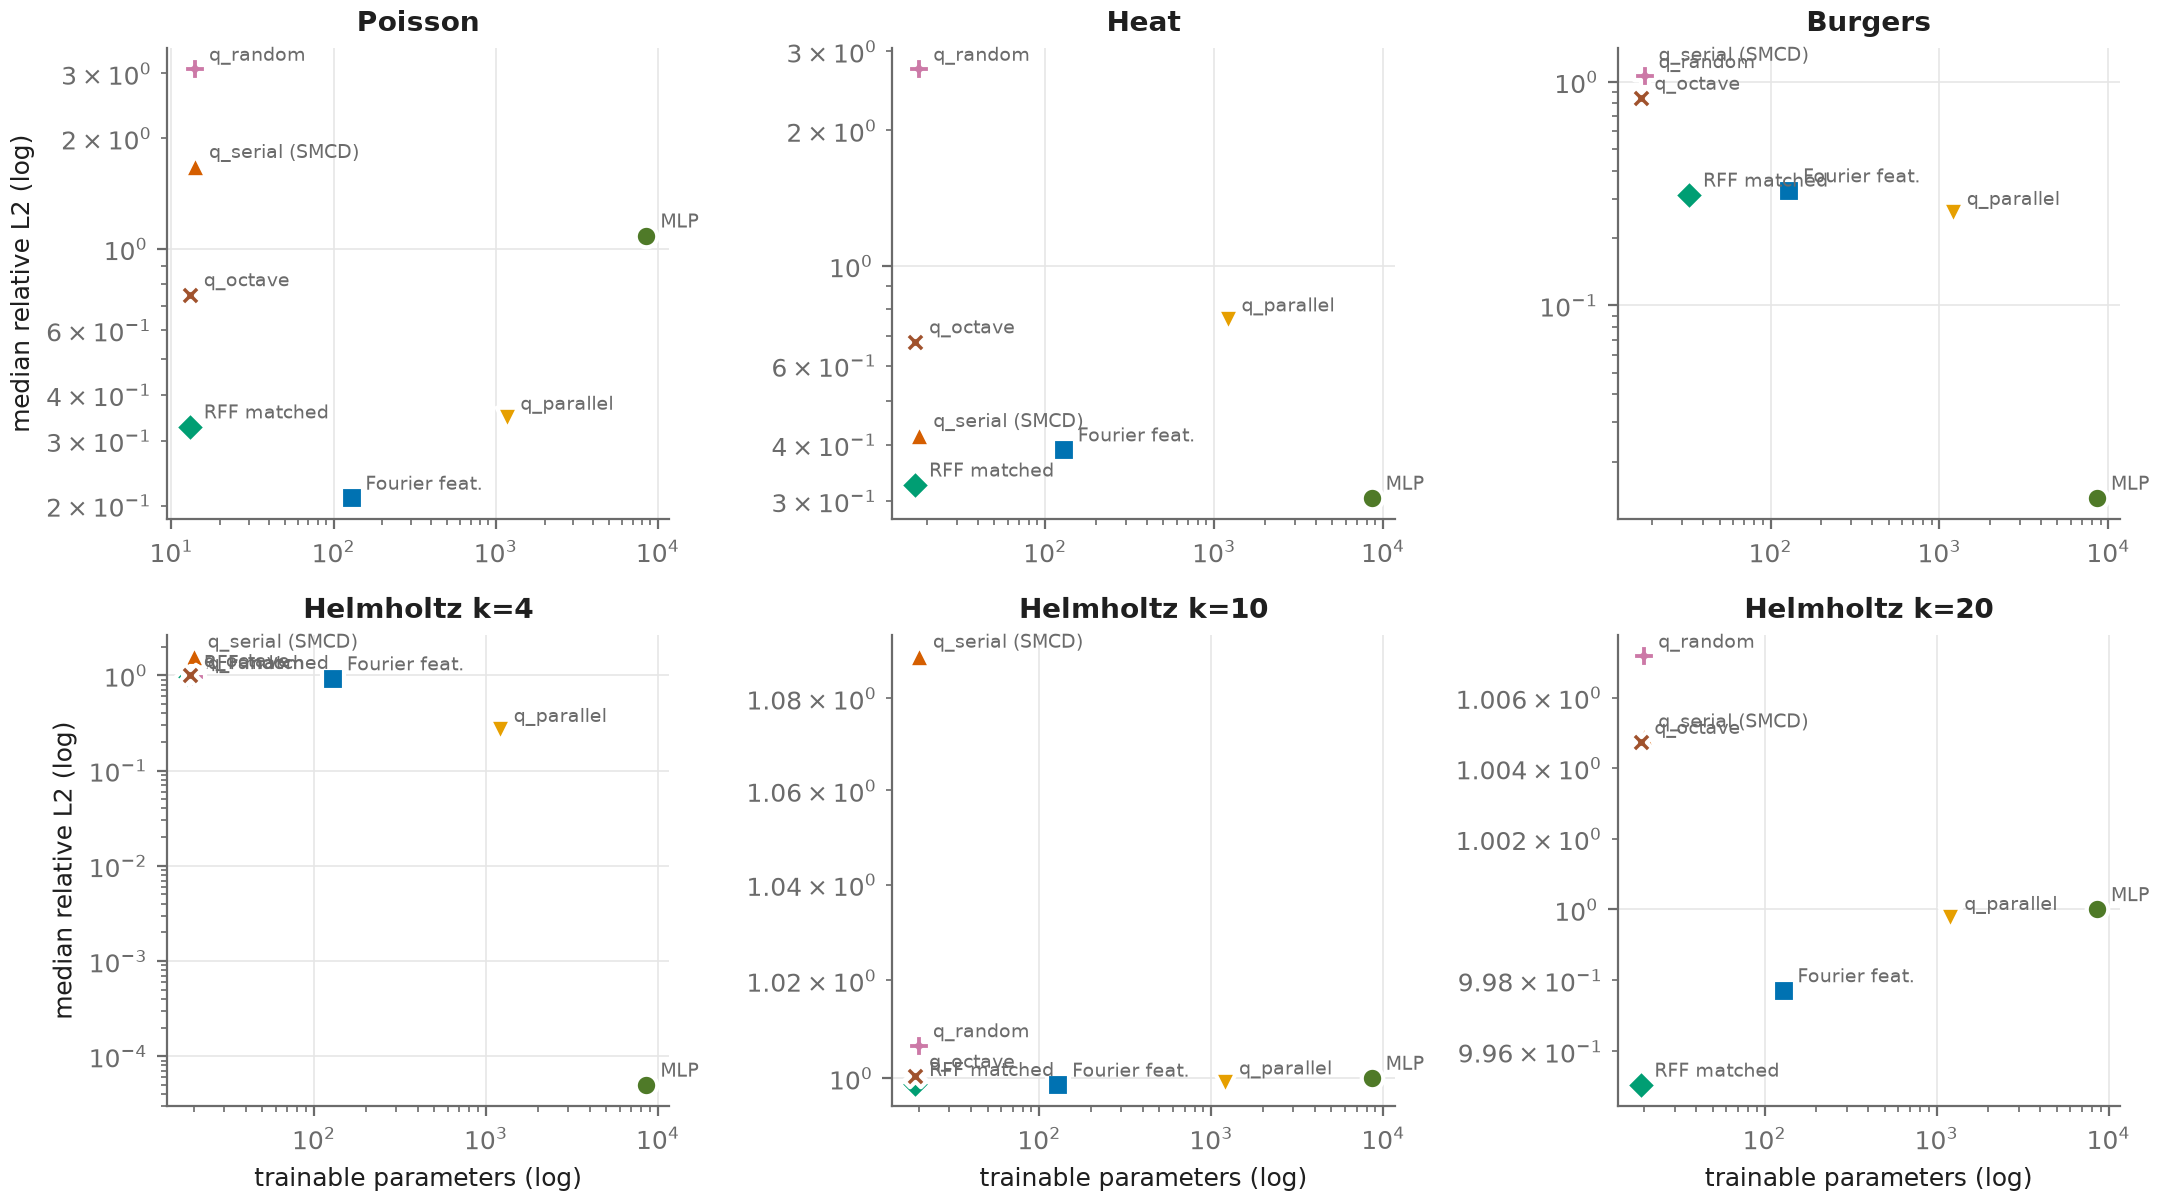
\includegraphics[width=0.49\linewidth]{../results/report/figures/cost_vs_accuracy_params.png}\hfill
  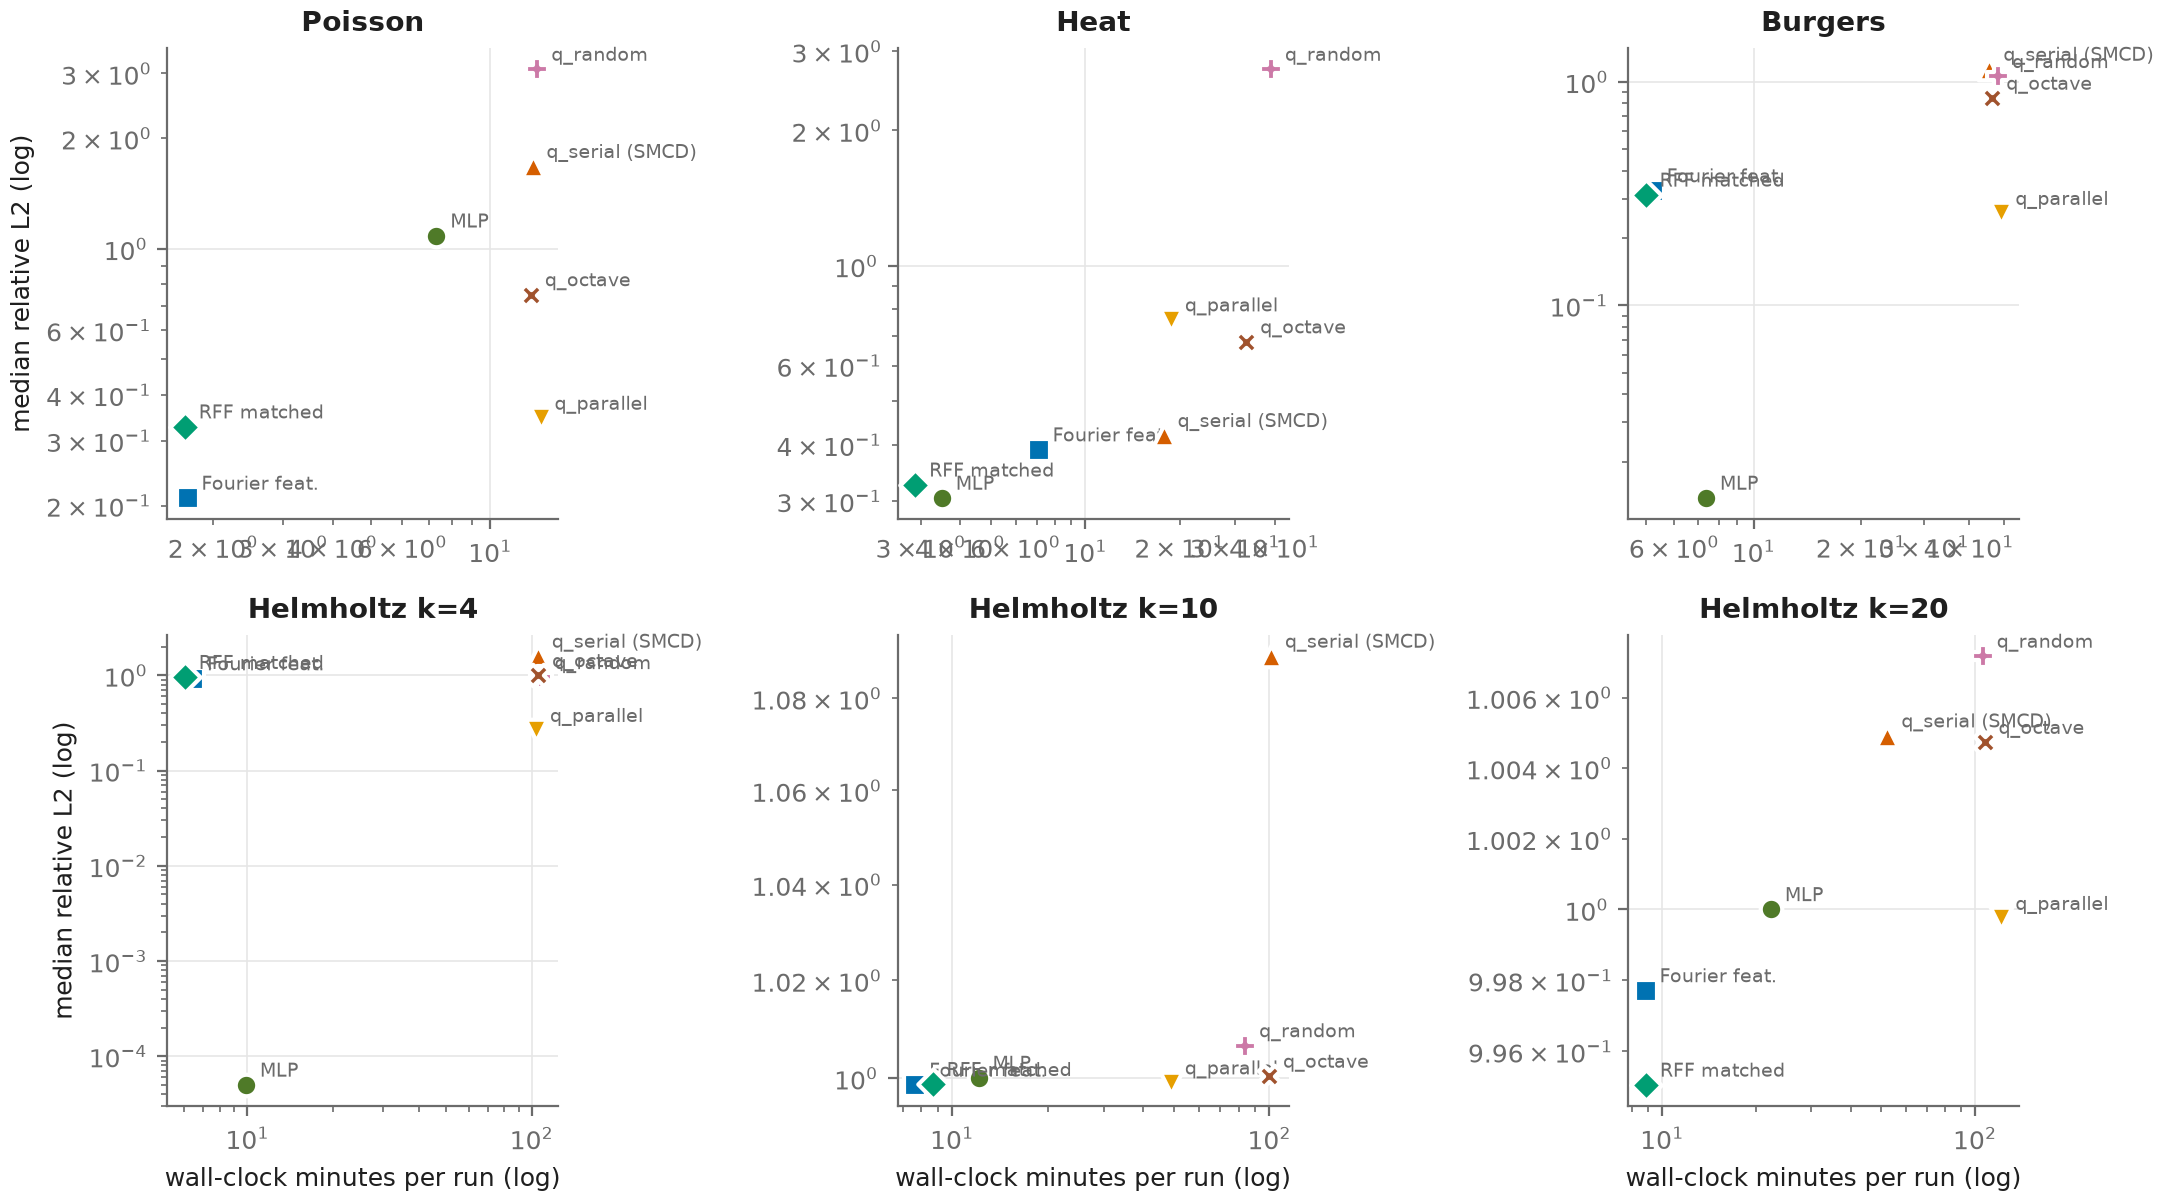
\includegraphics[width=0.49\linewidth]{../results/report/figures/cost_vs_accuracy_wallclock.png}
  \caption{Median error against parameter count (left) and wall-clock time per run
    (right), per problem.}
  \label{fig:cost}
\end{figure}

\begin{figure}[htbp]
  \centering
  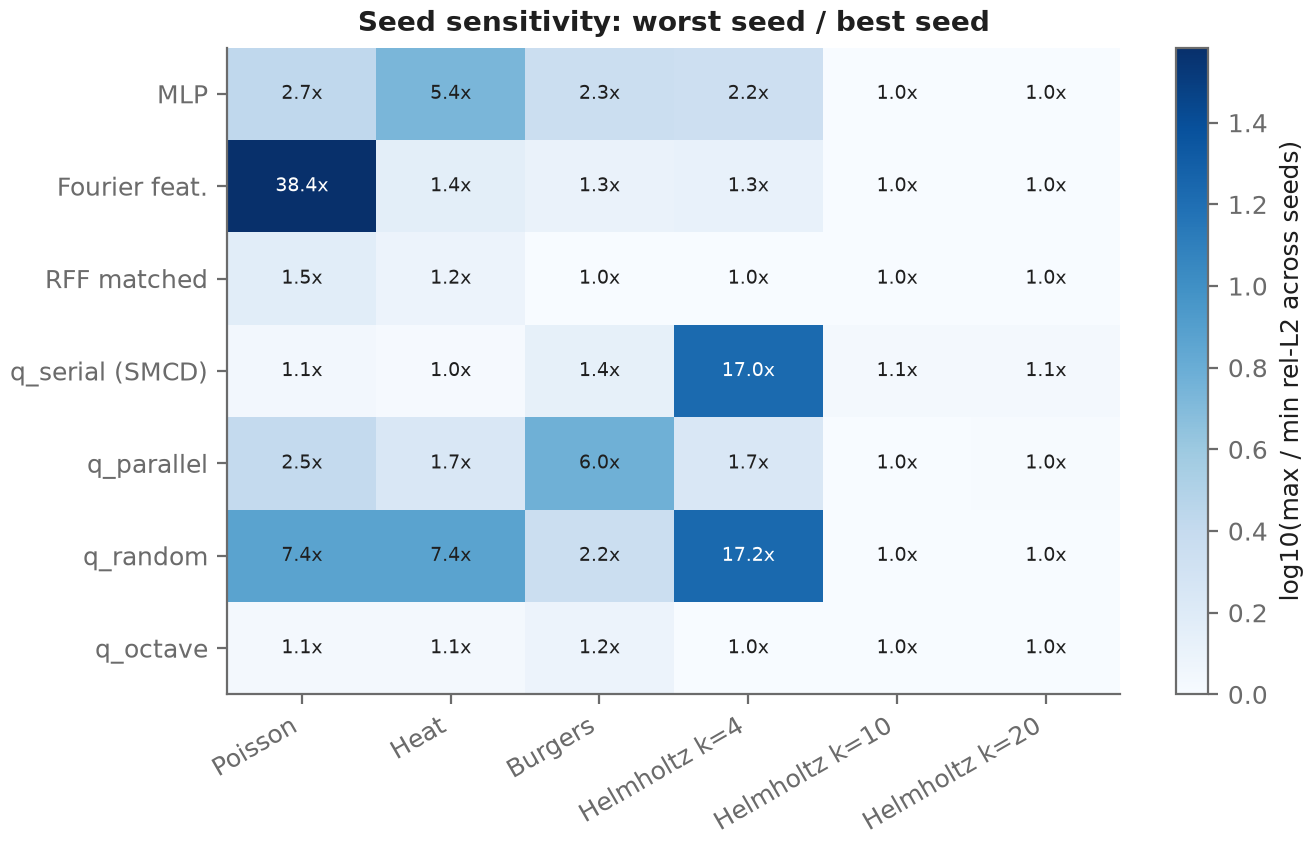
\includegraphics[width=0.7\linewidth]{../results/report/figures/seed_spread.png}
  \caption{Seed sensitivity: worst-seed over best-seed error for each family and problem.}
  \label{fig:seedspread}
\end{figure}

\begin{figure}[htbp]
  \centering
  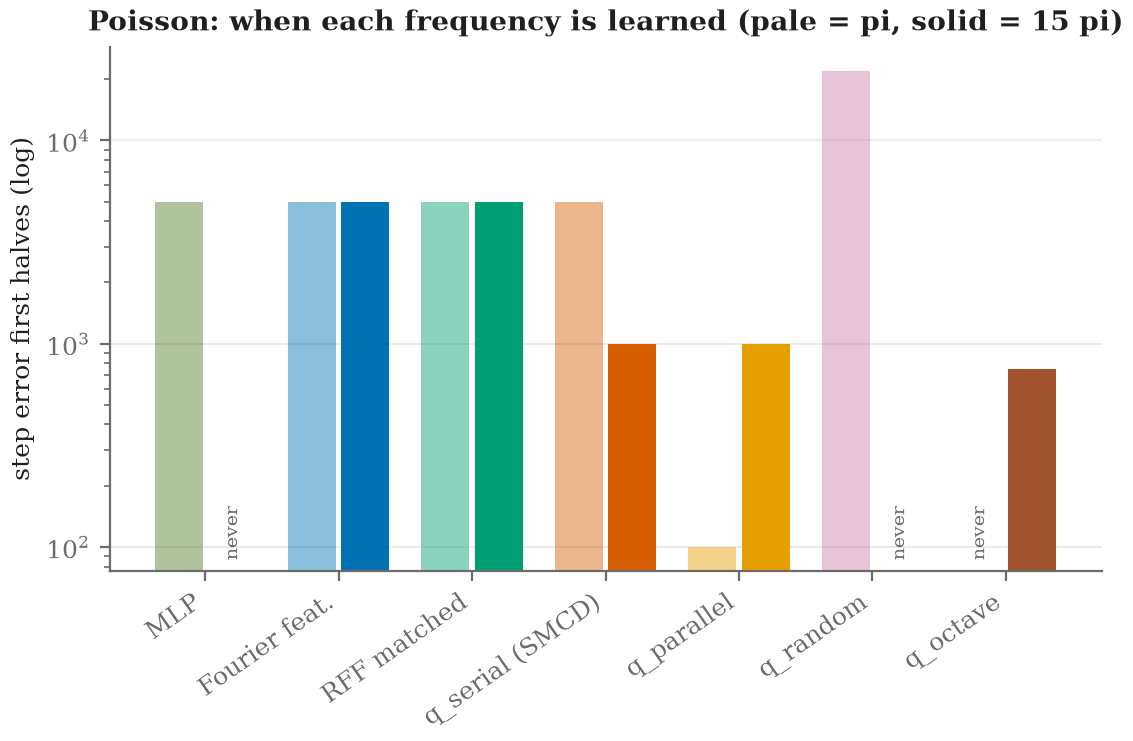
\includegraphics[width=0.49\linewidth]{../results/report/figures/xai_frequency_learning_order_poisson.png}\hfill
  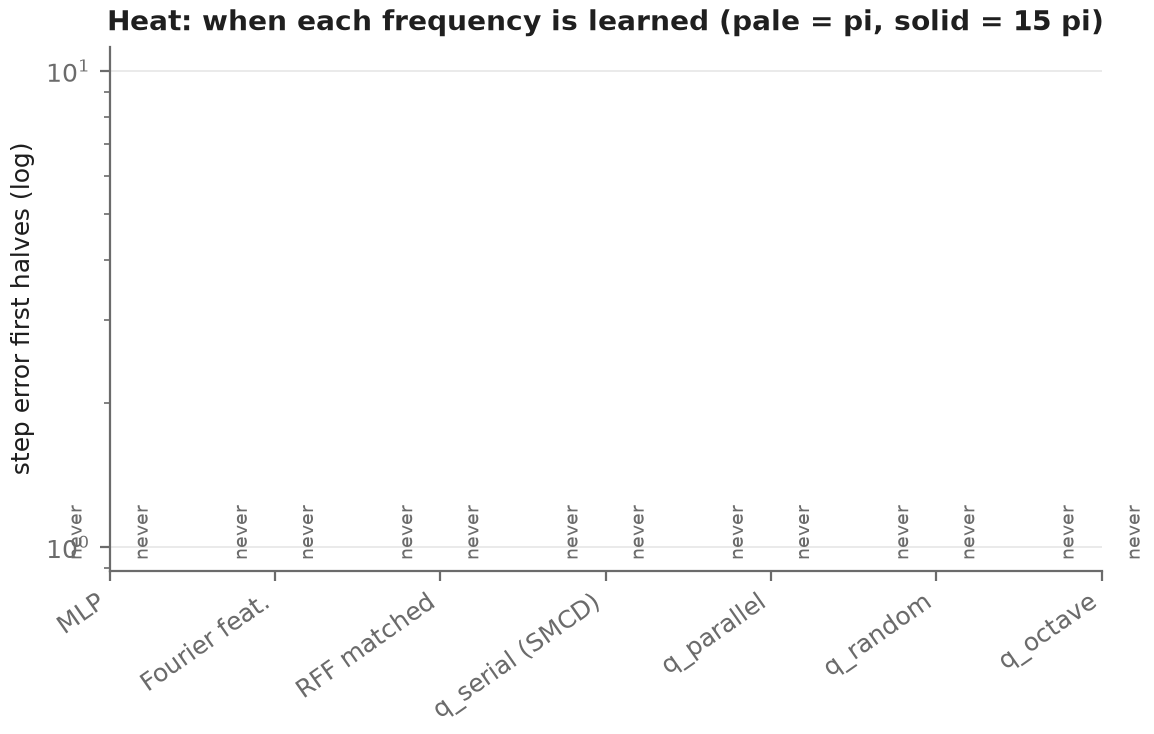
\includegraphics[width=0.49\linewidth]{../results/report/figures/xai_frequency_learning_order_heat.png}
  \caption{Step at which the error at each solution frequency first halves (median over
    seeds; pale: $\pi$, solid: $15\pi$). Left: Poisson; right: heat.}
  \label{fig:learnorder}
\end{figure}

\begin{figure}[htbp]
  \centering
  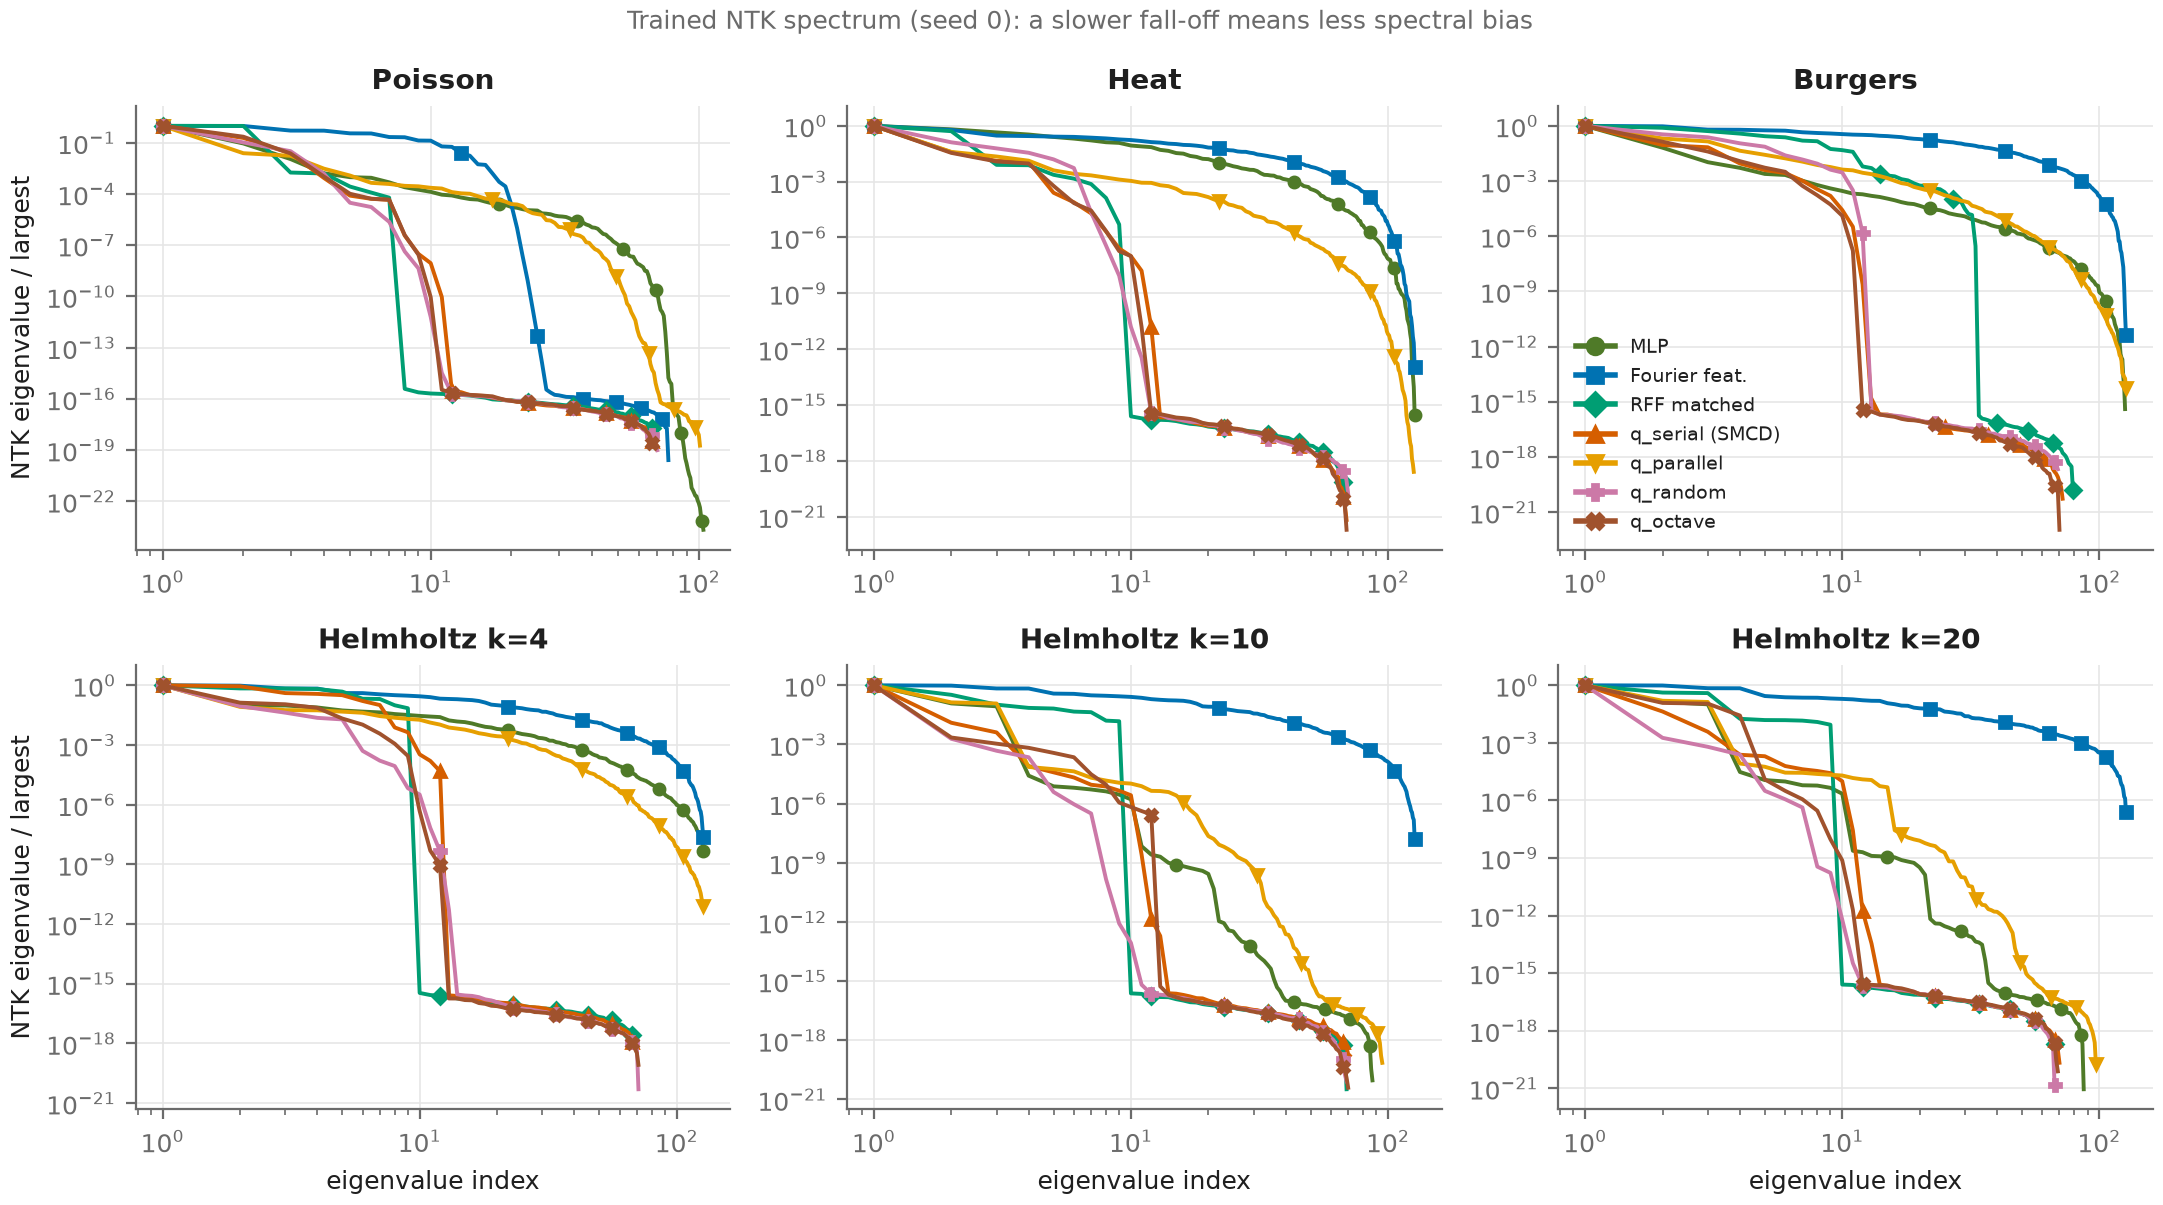
\includegraphics[width=\linewidth]{../results/report/figures/xai_ntk_spectra.png}
  \caption{Trained NTK spectra (seed 0), normalised by the largest eigenvalue.}
  \label{fig:ntkgallery}
\end{figure}

\begin{figure}[htbp]
  \centering
  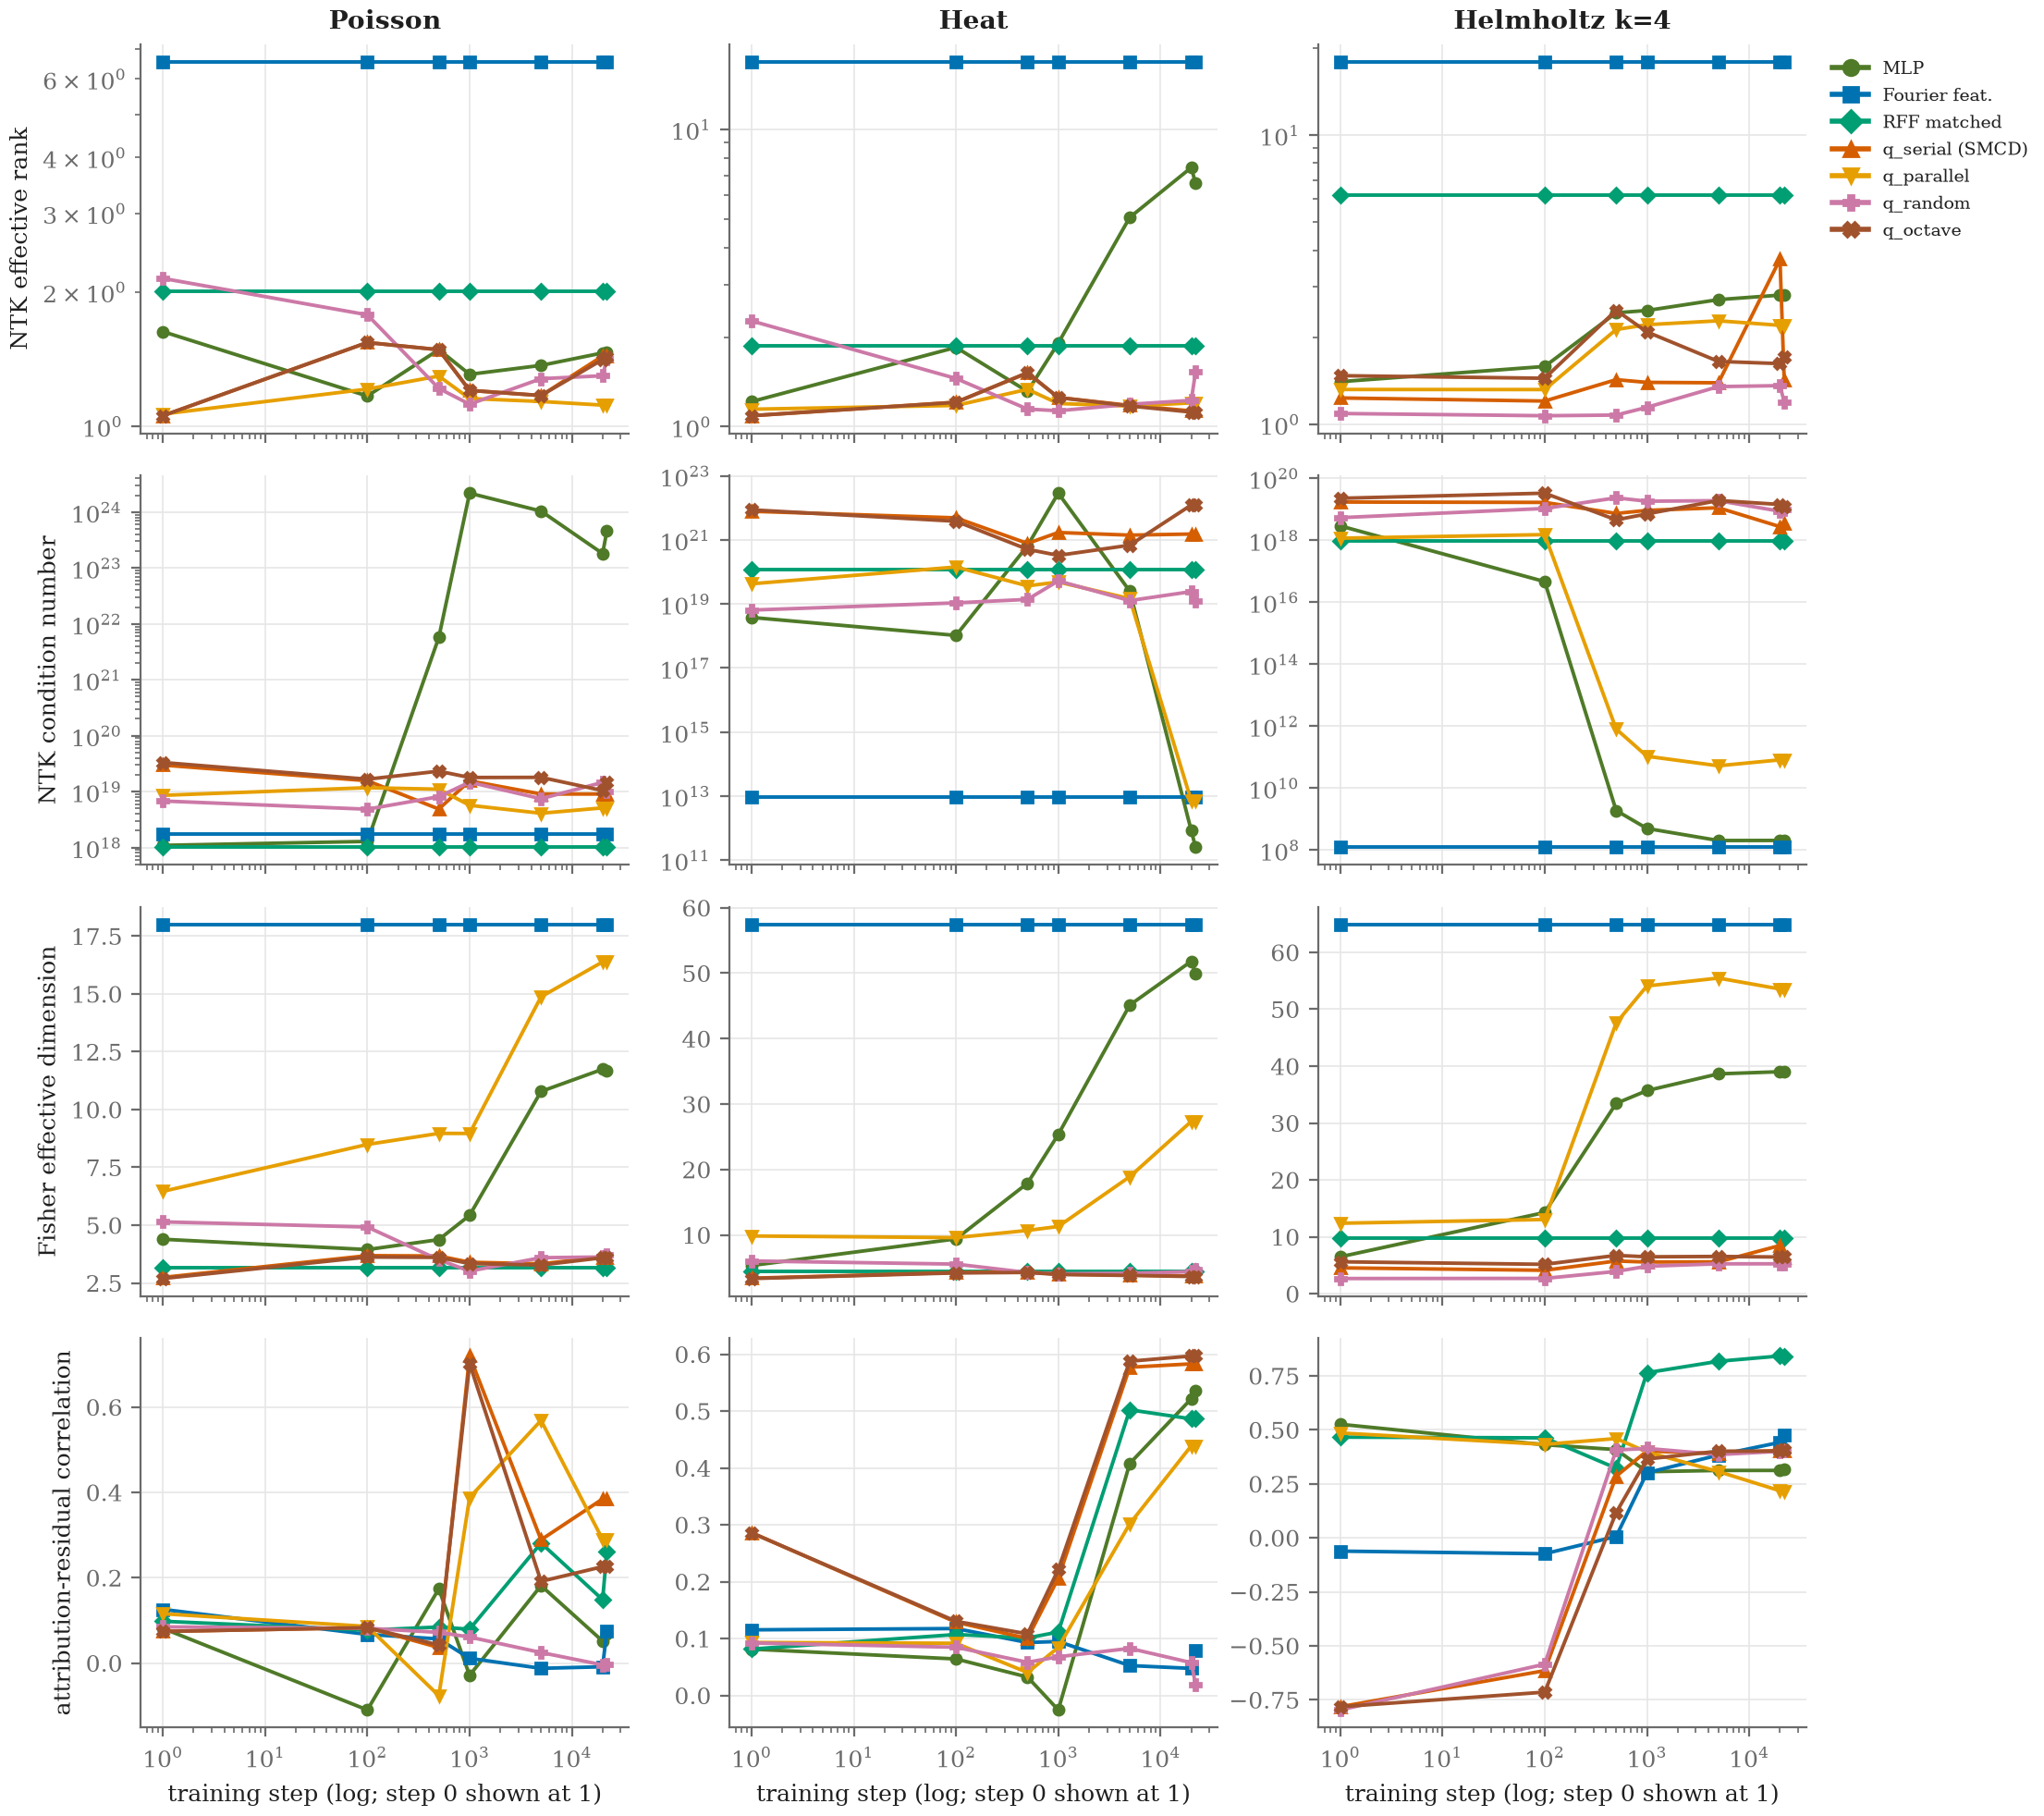
\includegraphics[width=0.95\linewidth]{../results/report/figures/xai_instrument_evolution.png}
  \caption{NTK effective rank and condition number, Fisher effective dimension and the
    correlation of attributions with the residual, over training (median over seeds).}
  \label{fig:evolution}
\end{figure}

\begin{figure}[htbp]
  \centering
  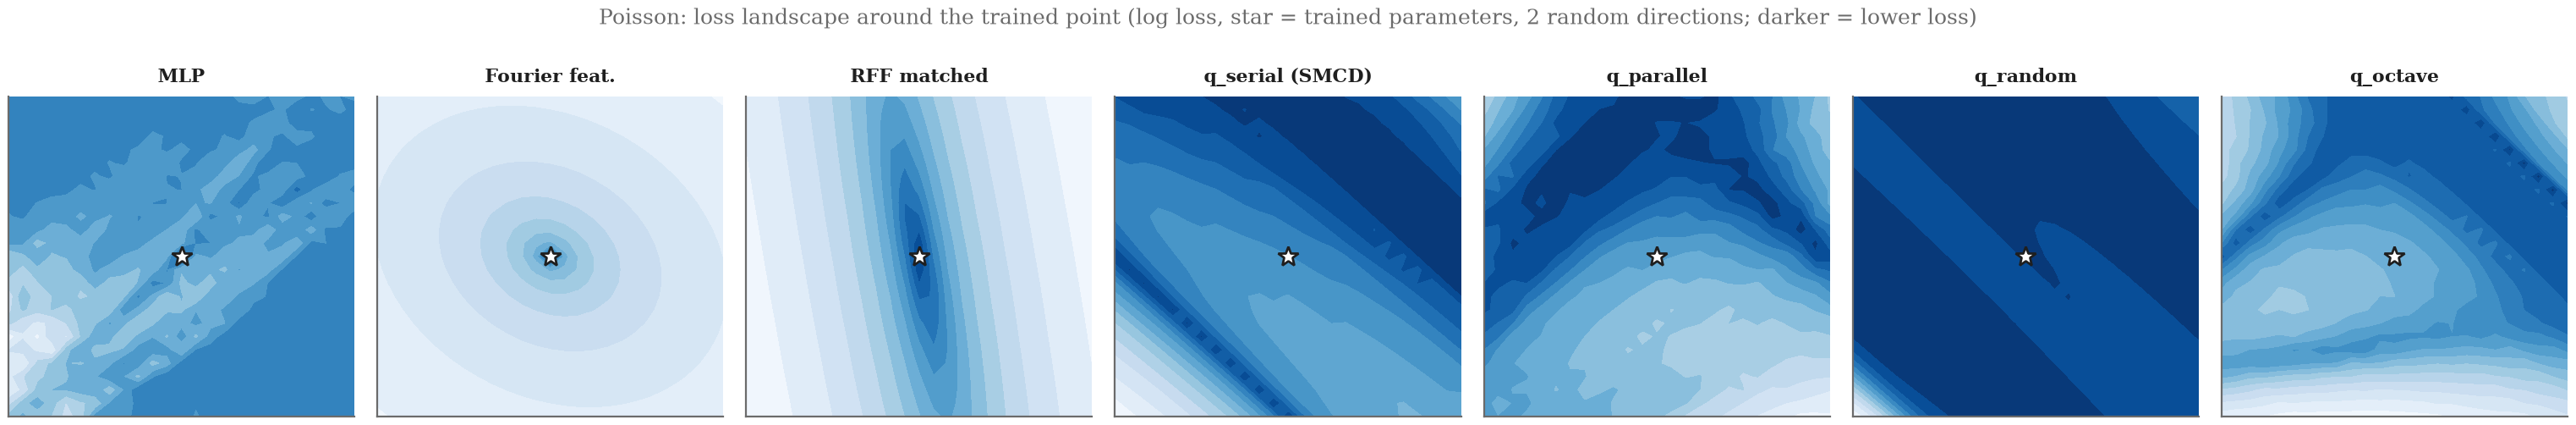
\includegraphics[width=\linewidth]{../results/report/figures/xai_landscapes_poisson.png}\\[4pt]
  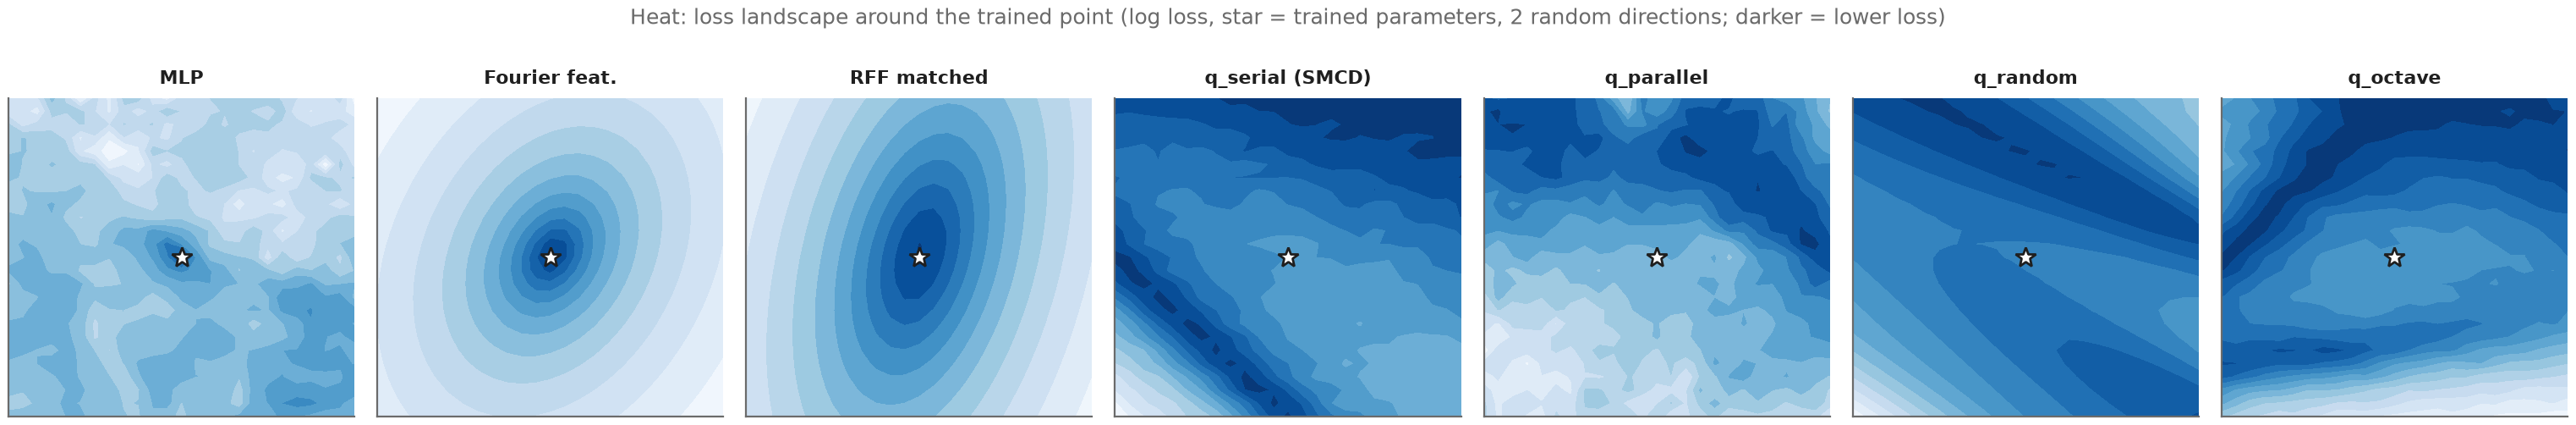
\includegraphics[width=\linewidth]{../results/report/figures/xai_landscapes_heat.png}
  \caption{Loss landscape on two random directions around the trained parameters (star),
    Poisson (top) and heat (bottom); darker is lower loss.}
  \label{fig:landscapes}
\end{figure}

\begin{figure}[htbp]
  \centering
  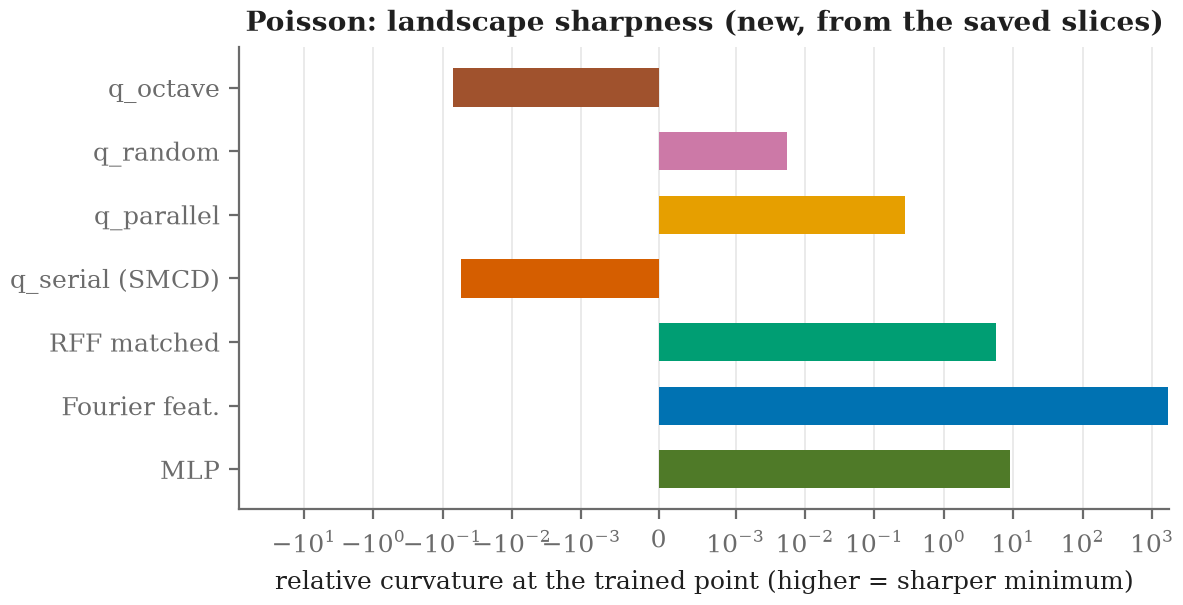
\includegraphics[width=0.49\linewidth]{../results/report/figures/xai_sharpness_poisson.png}\hfill
  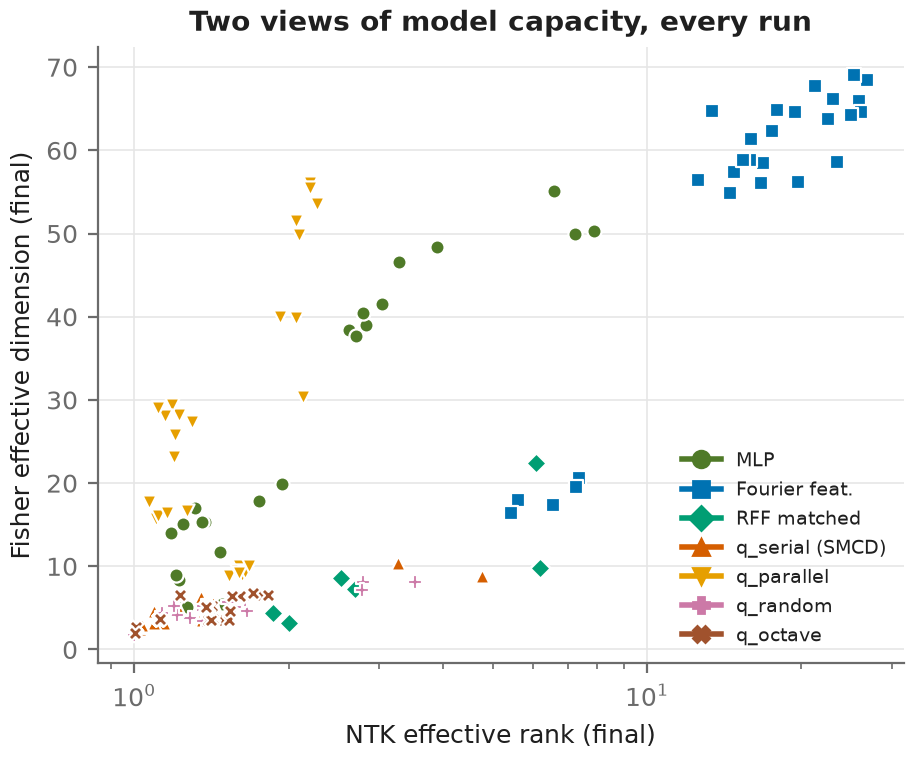
\includegraphics[width=0.49\linewidth]{../results/report/figures/xai_ntk_vs_fisher.png}
  \caption{Left: curvature of the loss landscape at the trained point (Poisson). Right:
    NTK effective rank against Fisher effective dimension, every run.}
  \label{fig:sharpness}
\end{figure}

\begin{figure}[htbp]
  \centering
  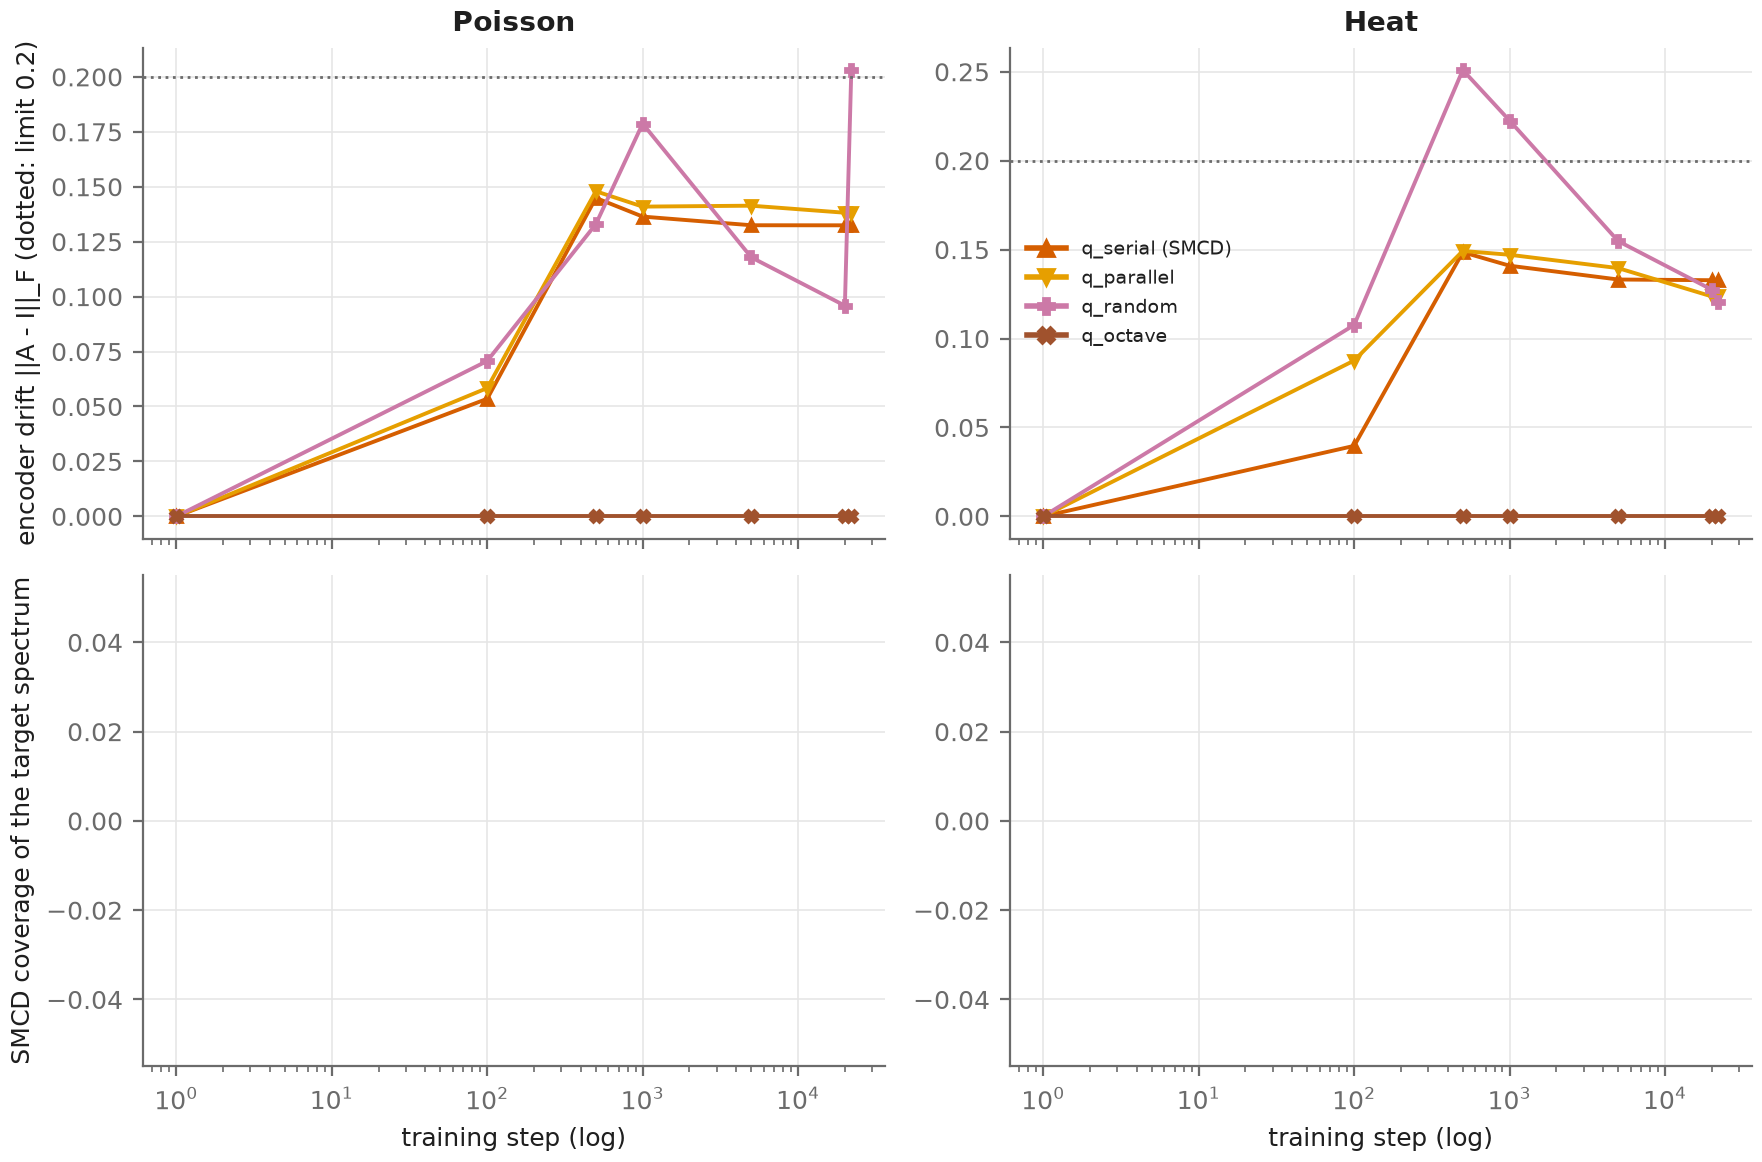
\includegraphics[width=0.85\linewidth]{../results/report/figures/xai_quantum_internals.png}
  \caption{Quantum families: encoder drift $\|A-I\|_F$ (dotted: the 0.2 limit) and
    SMCD coverage of the target spectrum over training.}
  \label{fig:qinternals}
\end{figure}

\begin{figure}[htbp]
  \centering
  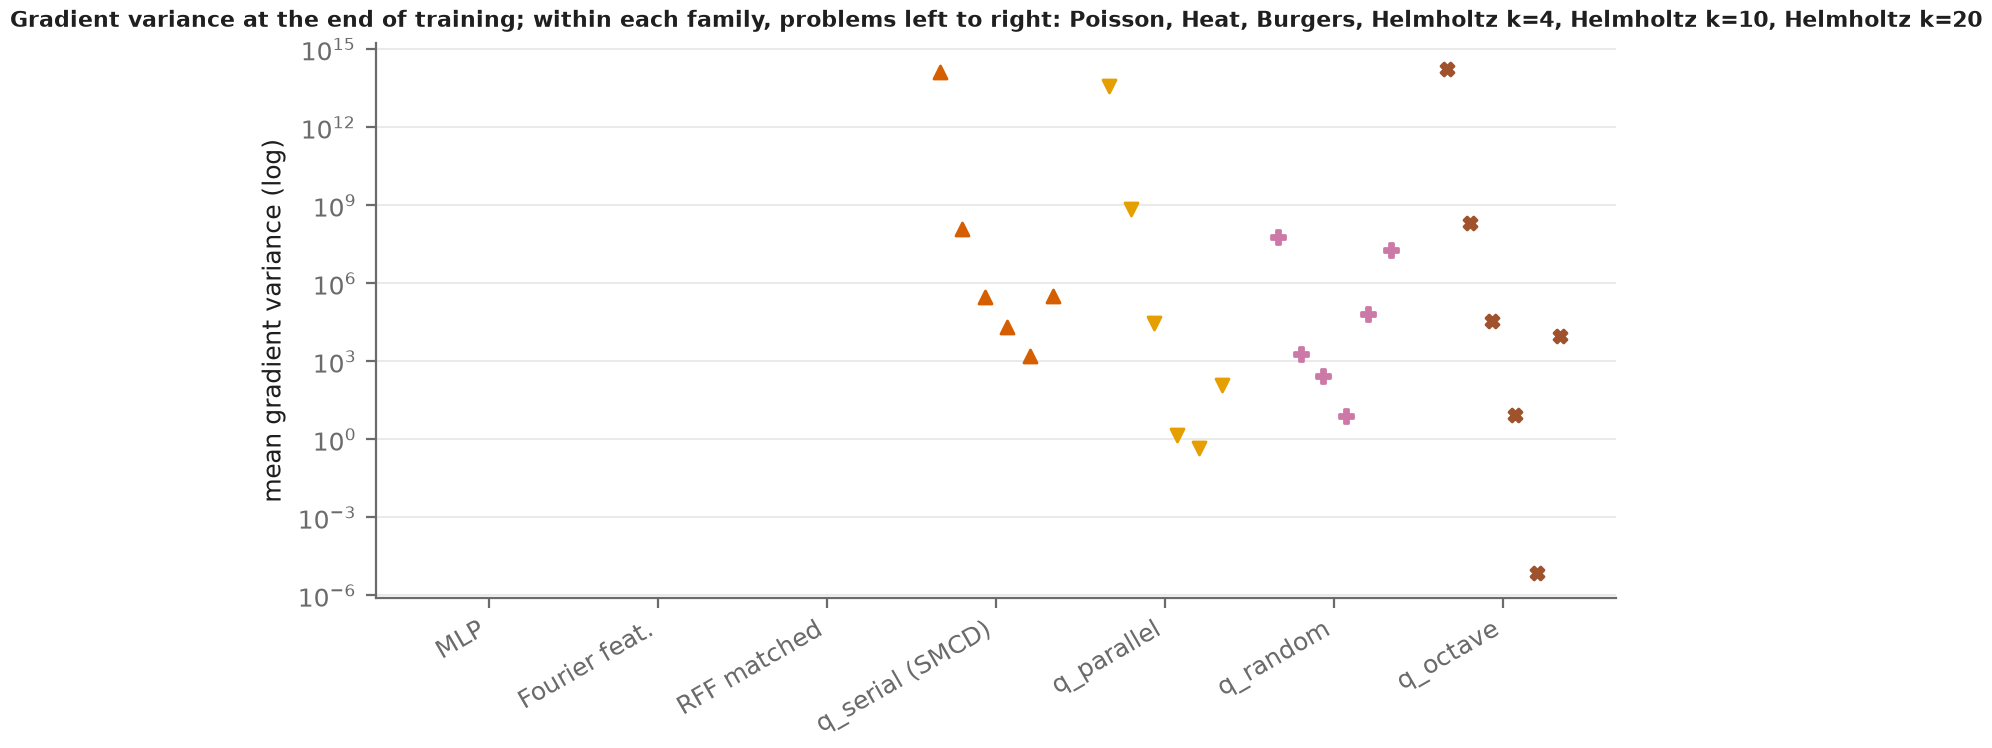
\includegraphics[width=0.8\linewidth]{../results/report/figures/xai_gradient_variance.png}
  \caption{Mean gradient variance at the end of training, per family and problem.}
  \label{fig:gradvar}
\end{figure}

\begin{figure}[htbp]
  \centering
  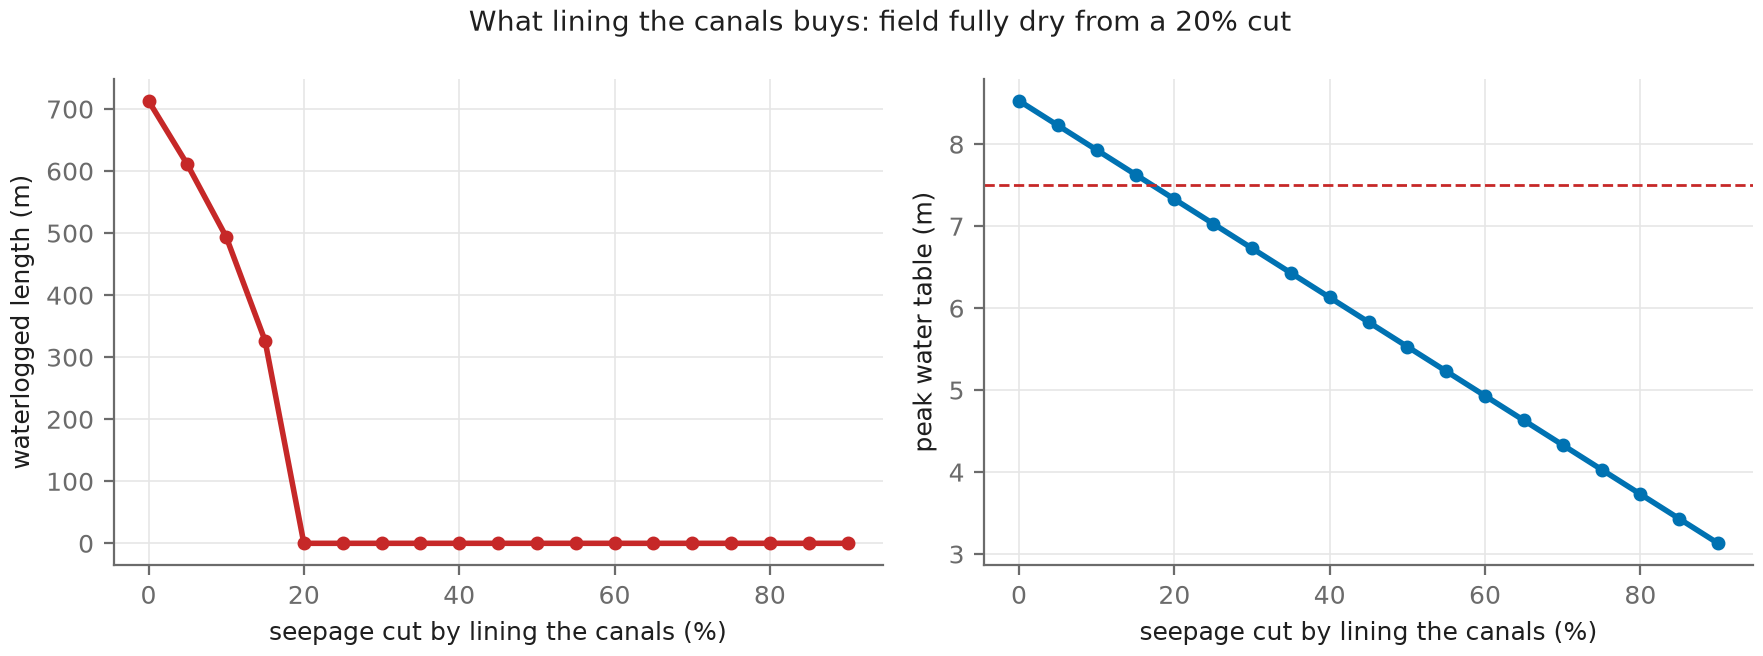
\includegraphics[width=0.49\linewidth]{../results/report/figures/groundwater_canal_lining.png}\hfill
  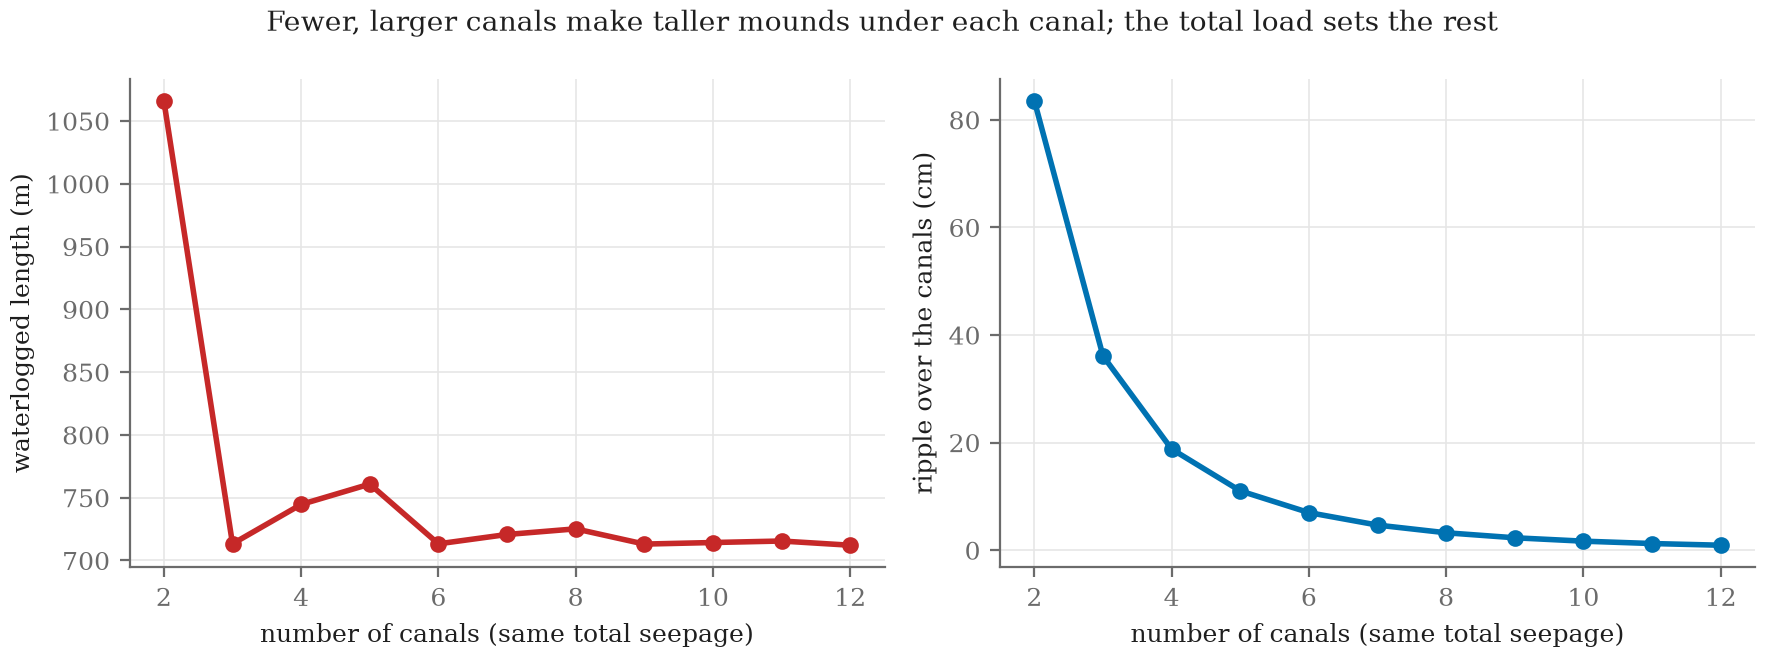
\includegraphics[width=0.49\linewidth]{../results/report/figures/groundwater_canal_spacing.png}\\[4pt]
  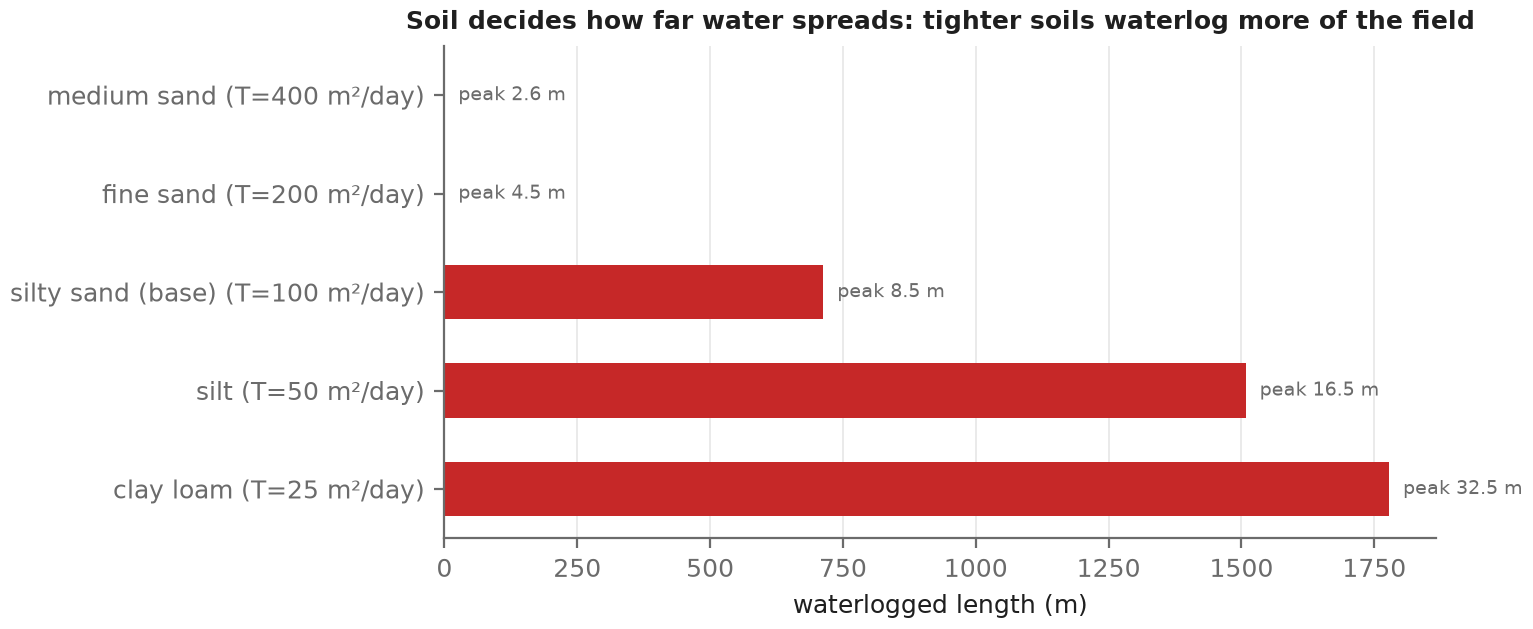
\includegraphics[width=0.6\linewidth]{../results/report/figures/groundwater_soil_type.png}
  \caption{Groundwater scenarios from the exact solution: lining the canals, canal
    spacing at the same total seepage, and soil type.}
  \label{fig:gwgallery}
\end{figure}
